% !TeX root = ./slides.tex

\documentclass{beamer}
\usepackage{datetime}
\usepackage{mathtools}
\usepackage{amsmath}
\usepackage{amsfonts}
\usepackage{amsthm}
\usepackage{amssymb}

\theoremstyle{plain}
\newtheorem{thm}{Theorem}
\newtheorem{lem}[thm]{Lemma}
\newtheorem{prop}[thm]{Proposition}
\newtheorem*{cor}{Corollary}

\theoremstyle{definition}
\newtheorem{defn}{Definition}
\newtheorem{conj}{Conjecture}
\newtheorem{exmp}{Example}

\theoremstyle{remark}
\newtheorem*{rem}{Remark}
\usepackage{floatrow}

\newenvironment{tzfigure}[1]
{
    \begin{figure}[ht]
        \centering
        #1
        \begin{tikzpicture}
}
{
        \end{tikzpicture}   
    \end{figure}
}

\newenvironment{tzcategory}[1]
{
    \begin{figure}[ht]
        \centering
        #1
        \begin{tikzpicture}[baseline= (a).base]    
}
{
    \end{tikzpicture}   
\end{figure}
}

\newenvironment{subtzcategory}[2]
{
    \begin{subfigure}[ht]{#2}
        \centering
        #1
        \begin{tikzpicture}[baseline= (a).base]    
}
{
    \end{tikzpicture}   
\end{subfigure}
}

\usepackage{graphicx}
\usepackage{caption}
\usepackage{subcaption}
\usepackage{tikz}
\usetikzlibrary{arrows,decorations.markings}
\usetikzlibrary{cd}
\usetikzlibrary{shapes.geometric,fit}
\usetikzlibrary{positioning}
\usepackage{etoolbox}
\listadd{\pc}{\footnotesize$C$}
\listadd{\pc}{\footnotesize$C\sharp$}
\listadd{\pc}{\footnotesize$D$}
\listadd{\pc}{\footnotesize$E\flat$}
\listadd{\pc}{\footnotesize$E$}
\listadd{\pc}{\footnotesize$F$}
\listadd{\pc}{\footnotesize$F\sharp$}
\listadd{\pc}{\footnotesize$G$}
\listadd{\pc}{\footnotesize$G\sharp$}
\listadd{\pc}{\footnotesize$A$}
\listadd{\pc}{\footnotesize$B\flat$}
\listadd{\pc}{\footnotesize$B$}



\usetheme{Singapore}
\usecolortheme{rose}
\usefonttheme{structurebold}
\usebackgroundtemplate{\includegraphics[width=\paperwidth]{./img/background.jpg}}


\setbeamertemplate{navigation symbols}{}
\AtBeginSection[]
{
	\begin{frame}
		\frametitle{Overview}
		\tableofcontents[currentsection]
    \end{frame}
}
\setbeamertemplate{footline}[page number]


\title{EK-nets}
\subtitle{Musical Constraints in Category Theory}
\author{Alice Rixte}
\institute[IRCAM]{ENS Paris-Saclay, IRCAM, CNRS, Sorbonne Université}
\newdate{date}{17}{09}{2020}
\date{\displaydate{date}}


\newcounter{itemcount}

\begin{document}
\begin{frame}
	\titlepage
\end{frame}

\begin{frame}
	\frametitle{Table of contents}
	\tableofcontents
\end{frame}

\section{Introduction}

\subsubsection{Transformational music theory}
\begin{frame}[fragile]
	\frametitle{Transformational music theory}
	\begin{itemize}
		\item Main focus : relations between musical objects
		\item Main tool : T/I group (dihedral group with 24 elements)
	\end{itemize}
	\begin{figure}
		\begin{subfigure}[c]{.27\textwidth}
			\centering
			\setcounter{itemcount}{450}
			\renewcommand*{\do}[1]{
				\filldraw [black](\number\value{itemcount}:3cm)
				circle (1.5pt)
				node[anchor={\number\value{itemcount}-180}]
					{#1\addtocounter{itemcount}{-30}};}
			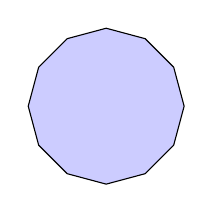
\begin{tikzpicture}[scale=0.33]
				\dolistloop{\pc}
				\draw[fill=blue!20] (90:3cm) -- (60:3cm) -- (30:3cm) -- (0:3cm) --  (330:3cm) -- (300:3cm) -- (270:3cm) -- (240:3cm) -- (210:3cm) -- (180 :3cm) -- (150:3cm) -- (120:3cm) -- cycle;
			\end{tikzpicture}
			\caption{Pitch-classes dodecahedron}
			\label{fig:dode-id}
		\end{subfigure}%
		\hspace{0.2cm}{\color{blue!40}\LARGE$\xRightarrow{T_2}$}\hspace{0cm}%
		\begin{subfigure}[c]{.27\textwidth}
			\centering
			\setcounter{itemcount}{510}
			\renewcommand*{\do}[1]{
				\filldraw [black](\number\value{itemcount}:3cm)
				circle (1.5pt)
				node[anchor={\number\value{itemcount}-180}]
					{#1\addtocounter{itemcount}{-30}};}
			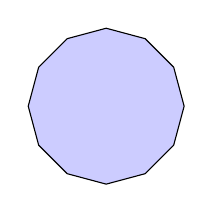
\begin{tikzpicture}[scale=0.33]
				\dolistloop{\pc}
				\draw[fill=blue!20] (90:3cm) -- (60:3cm) -- (30:3cm) -- (0:3cm) --  (330:3cm) -- (300:3cm) -- (270:3cm) -- (240:3cm) -- (210:3cm) -- (180 :3cm) -- (150:3cm) -- (120:3cm) -- cycle;
			\end{tikzpicture}
			\caption{Transposition of 2 semi-tones (Rotation)}
			\label{fig:dode-T2}
		\end{subfigure}%
		\hspace{0.2cm}{\color{purple}\LARGE$\xRightarrow{I_4}$}\hspace{0cm}%
		\begin{subfigure}[c]{.27\textwidth}
			\centering
			\setcounter{itemcount}{510}
			\renewcommand*{\do}[1]{
				\filldraw [black](\number\value{itemcount}:3cm)
				circle (1.5pt)
				node[anchor={\number\value{itemcount}-180}]
					{#1\addtocounter{itemcount}{30}};}
			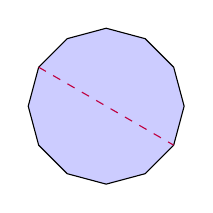
\begin{tikzpicture}[scale=0.33]

				\dolistloop{\pc}
				\draw[fill=blue!20] (90:3cm) -- (60:3cm) -- (30:3cm) -- (0:3cm) --  (330:3cm) -- (300:3cm) -- (270:3cm) -- (240:3cm) -- (210:3cm) -- (180 :3cm) -- (150:3cm) -- (120:3cm) -- cycle;
				\draw[purple,dashed] (150:3cm) -- (330:3cm);
			\end{tikzpicture}
			\caption{$4^{th}$ inversion  (Symmetry)}
			\label{fig:dode-I4}
		\end{subfigure}%
		\caption{Transpositions and inversions in a dodecahedron}
		\label{fig:dode-TI}
	\end{figure}

\end{frame}

\subsubsection{K-nets : using the T/I group}


\begin{frame}[fragile]
	\frametitle{K-nets : using the T/I group}
	\begin{columns}
		\begin{column}{0.4\textwidth}
			\begin{column}{0.85\textwidth}

				\begin{figure}
					\centering

					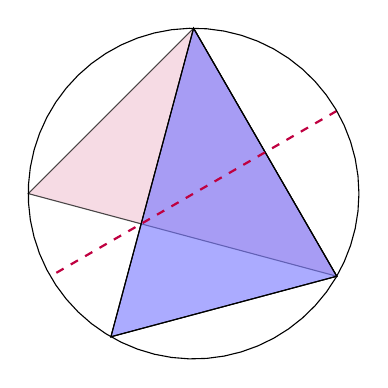
\begin{tikzpicture}[scale=0.7]
						\setcounter{itemcount}{450}
						\renewcommand*{\do}[1]{
							\filldraw [black](\number\value{itemcount}:3cm)
							circle (1.5pt)
							node[anchor={\number\value{itemcount}-180}]
								{#1\addtocounter{itemcount}{-30}};}

						\dolistloop{\pc}
						\draw[fill=purple!20,opacity=0.7] (90:3cm) -- (330:3cm) -- (180:3cm) -- cycle;
						\draw[fill=blue!55, fill opacity=0.6] (90:3cm) -- (330:3cm) -- (240:3cm) -- cycle;
						\draw (90:3cm) -- (330:3cm) -- (240:3cm) -- cycle;
						\draw [dashed, thick, purple, opacity=1] (30:3cm) -- (210:3cm);
						\draw [domain=0:360,samples=60] plot ({3*cos(\x)}, {3*sin(\x)});

					\end{tikzpicture}
					\caption{The $I_4$ inversion on the C major chord}
					\label{fig:Rtransf}
				\end{figure}
			\end{column}

		\end{column}
		\pause
		\begin{column}{0.52\textwidth}
			\begin{equation*}F\big<11,4\big> =
				\left\{ \begin{aligned}
					T_i & \rightarrow T_{11i}   = T_{-i}     \\
					I_j & \rightarrow I_{11j+4} = T_{-j + 4} \\
				\end{aligned} \right.
			\end{equation*}

			\vspace{0cm}

			\begin{figure}[t]

				\begin{subfigure}{.46\textwidth}
					\centering
					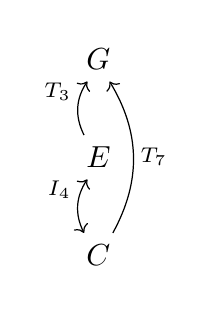
\begin{tikzpicture}
						% https://tikzcd.yichuanshen.de/#N4Igdg9gJgpgziAXAbVABwnAlgFyxMJZABgBoAmAXVJADcBDAGwFcYkQBhEAX1PU1z5CKMgEZqdJq3YBRHnxAZseAkTLEJDFm0QgA4jwkwoAc3hFQAMwBOEALZIyIHBCSiaAIxhgoSAMxOWtK6ACoA+gAs8la2Dojuzq6I5J7evogBNEE6IOF+0SA29o40LkgpIF4+SAC0mc70WIzskGBsNHAAFliWOCUgjPRejAAKAirCINZYJp19WVI5AJJhAOyG3EA
						\node[scale=1.1] (a) at (0,0){
							\begin{tikzcd}
								G\\
								E \arrow[u, "T_3", bend left]\\
								C \arrow[u, "I_4",leftrightarrow, bend left]
								\arrow[uu, "T_7"',  bend right]
							\end{tikzcd}
						};
					\end{tikzpicture}
					\caption{C K-net}
					\label{fig:KCmajor}
				\end{subfigure}%
				%\hspace{-0.2cm}%
				{\Large$\xRightarrow{\text%
						{\scriptsize $F\big< 11,4 \big>$}}$}%
				%\hspace{-0.2cm}%
				\begin{subfigure}{.50\textwidth}
					\centering

					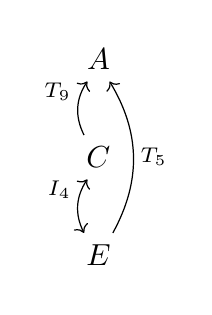
\begin{tikzpicture}

						% https://tikzcd.yichuanshen.de/#N4Igdg9gJgpgziAXAbVABwnAlgFyxMJZABgBoAmAXVJADcBDAGwFcYkQBhEAX1PU1z5CKMgEZqdJq3YBRHnxAZseAkTLEJDFm0QgA4jwkwoAc3hFQAMwBOEALZIyIHBCSiaAIxhgoSAMxOWtK6ACoA+gAs8la2Dojuzq6I5J7evogBNEE6IOF+0SA29o40LkgpIF4+SAC0mc70WIzskGBsNHAAFliWOCUgjPRejAAKAirCINZYJp19WVI5AJJhAOyG3EA
						\node[scale=1.1] (a) at (0,0){
							\begin{tikzcd}
								A \\
								C \arrow[u, "T_9", bend left]\\
								E \arrow[u, "I_4",leftrightarrow, bend left]
								\arrow[uu, "T_5"', bend right]
							\end{tikzcd}
						};
					\end{tikzpicture}
					\caption{Am K-net}
					\label{fig:KAminor}
				\end{subfigure}
				\caption{Isography between C and Am}
				\label{fig:Kisography}
			\end{figure}
		\end{column}
	\end{columns}
\end{frame}





\subsubsection{K-nets are not always correct}
\begin{frame}[fragile]
	\frametitle{K-nets are not always sound}
	\begin{columns}
		\begin{column}{0.4\textwidth}
			\begin{itemize}
				\item \textbf{What is a "correct" K-net ?}
			\end{itemize}
			\begin{figure}
				\centering

				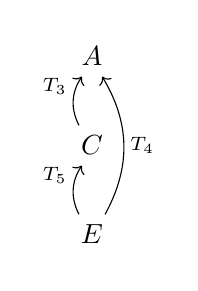
\begin{tikzpicture}

					% https://tikzcd.yichuanshen.de/#N4Igdg9gJgpgziAXAbVABwnAlgFyxMJZABgBoAmAXVJADcBDAGwFcYkQBhEAX1PU1z5CKMgEZqdJq3YBRHnxAZseAkTLEJDFm0QgA4jwkwoAc3hFQAMwBOEALZIyIHBCSiaAIxhgoSAMxOWtK6ACoA+gAs8la2Dojuzq6I5J7evogBNEE6IOF+0SA29o40LkgpIF4+SAC0mc70WIzskGBsNHAAFliWOCUgjPRejAAKAirCINZYJp19WVI5AJJhAOyG3EA
					\node[scale=1] (a) at (0,0){
						\begin{tikzcd}
							A \\
							C \arrow[u, "T_3", bend left]\\
							E \arrow[u, "T_5", bend left]
							\arrow[uu, "T_4"', bend right]
						\end{tikzcd}
					};
				\end{tikzpicture}
				\caption{Incorrect K-net}
				\label{fig:KAminor}
			\end{figure}
			Let us first decompose K-nets into 2 components.

		\end{column}
		\pause
		\begin{column}{0.65\textwidth}
			\begin{itemize}
				\item the pattern graph which may be of the form
			\end{itemize}
			\begin{figure}
				\centering

				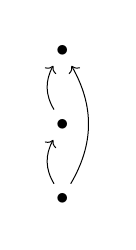
\begin{tikzpicture}

					% https://tikzcd.yichuanshen.de/#N4Igdg9gJgpgziAXAbVABwnAlgFyxMJZABgBoAmAXVJADcBDAGwFcYkQBhEAX1PU1z5CKMgEZqdJq3YBRHnxAZseAkTLEJDFm0QgA4jwkwoAc3hFQAMwBOEALZIyIHBCSiaAIxhgoSAMxOWtK6ACoA+gAs8la2Dojuzq6I5J7evogBNEE6IOF+0SA29o40LkgpIF4+SAC0mc70WIzskGBsNHAAFliWOCUgjPRejAAKAirCINZYJp19WVI5AJJhAOyG3EA
					\node[scale=0.9] (a) at (0,0){
						\begin{tikzcd}
							\bullet \\
							\bullet \arrow[u, "", bend left]\\
							\bullet \arrow[u, "", bend left]
							\arrow[uu, ""', bend right]
						\end{tikzcd}
					};
				\end{tikzpicture}
				\caption{Pattern of a K-net}
				\label{fig:KAminor}
			\end{figure}
			\begin{itemize}
				\item a labeling application F which associate an element of T/I to each arrow.
			\end{itemize}

		\end{column}
	\end{columns}

\end{frame}


\subsubsection{K-Isographies do not preserve correctness of K-nets}
\begin{frame}[fragile]
	\frametitle{K-Isographies do not preserve correctness of K-nets}
	\begin{columns}


		\begin{column}{0.4\textwidth}
			\begin{figure}[t]

				\begin{subfigure}{.46\textwidth}
					\centering
					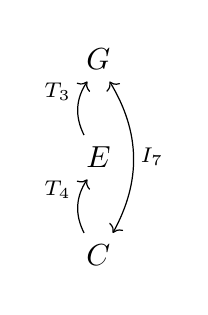
\begin{tikzpicture}
						% https://tikzcd.yichuanshen.de/#N4Igdg9gJgpgziAXAbVABwnAlgFyxMJZABgBoAmAXVJADcBDAGwFcYkQBhEAX1PU1z5CKMgEZqdJq3YBRHnxAZseAkTLEJDFm0QgA4jwkwoAc3hFQAMwBOEALZIyIHBCSiaAIxhgoSAMxOWtK6ACoA+gAs8la2Dojuzq6I5J7evogBNEE6IOF+0SA29o40LkgpIF4+SAC0mc70WIzskGBsNHAAFliWOCUgjPRejAAKAirCINZYJp19WVI5AJJhAOyG3EA
						\node[scale=1.1] (a) at (0,0){
							\begin{tikzcd}
								G\\
								E \arrow[u, "T_3", bend left]\\
								C \arrow[u, "T_4", bend left]
								\arrow[uu, "I_7"', leftrightarrow, bend right]
							\end{tikzcd}
						};
					\end{tikzpicture}
					\caption{C K-net}
					\label{fig:KCmajor}
				\end{subfigure}%
				%\hspace{-0.2cm}%
				{\Large$\xRightarrow{\text%
						{\scriptsize $F\big< 11,4 \big>$}}$}%
				%\hspace{-0.2cm}%
				\begin{subfigure}{.50\textwidth}
					\centering

					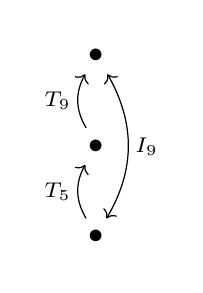
\begin{tikzpicture}

						% https://tikzcd.yichuanshen.de/#N4Igdg9gJgpgziAXAbVABwnAlgFyxMJZABgBoAmAXVJADcBDAGwFcYkQBhEAX1PU1z5CKMgEZqdJq3YBRHnxAZseAkTLEJDFm0QgA4jwkwoAc3hFQAMwBOEALZIyIHBCSiaAIxhgoSAMxOWtK6ACoA+gAs8la2Dojuzq6I5J7evogBNEE6IOF+0SA29o40LkgpIF4+SAC0mc70WIzskGBsNHAAFliWOCUgjPRejAAKAirCINZYJp19WVI5AJJhAOyG3EA
						\node[scale=1.1] (a) at (0,0){
							\begin{tikzcd}
								\bullet \\
								\bullet \arrow[u, "T_9", bend left]\\
								\bullet \arrow[u, "T_5", bend left]
								\arrow[uu, "I_9"',leftrightarrow, bend right]
							\end{tikzcd}
						};
					\end{tikzpicture}
					\caption{Incorrect K-net}
					\label{fig:KAminor}
				\end{subfigure}
				\caption{Isography between C and unsound K-net}
				\label{fig:Kisography}
			\end{figure}
		\end{column}
		\hspace{1cm}
		\begin{column}{0.6\textwidth}

			\begin{figure}
				\centering

				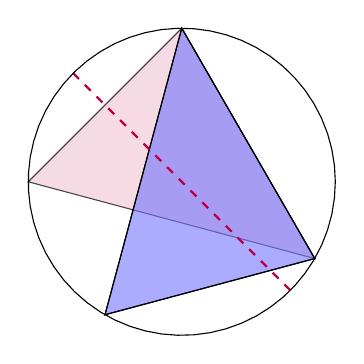
\begin{tikzpicture}[scale=0.65]
					\setcounter{itemcount}{450}
					\renewcommand*{\do}[1]{
						\filldraw [black](\number\value{itemcount}:3cm)
						circle (1.5pt)
						node[anchor={\number\value{itemcount}-180}]
							{#1\addtocounter{itemcount}{-30}};}

					\dolistloop{\pc}
					\draw[fill=purple!20,opacity=0.7] (90:3cm) -- (330:3cm) -- (180:3cm) -- cycle;
					\draw[fill=blue!55, fill opacity=0.6] (90:3cm) -- (330:3cm) -- (240:3cm) -- cycle;
					\draw (90:3cm) -- (330:3cm) -- (240:3cm) -- cycle;
					\draw [dashed, thick, purple, opacity=1] (315:3cm) -- (135:3cm);
					\draw [domain=0:360,samples=60] plot ({3*cos(\x)}, {3*sin(\x)});

				\end{tikzpicture}
				\caption{The symmetric of $E$ via $I_9$ is $F$ instead of $A$}
				\label{fig:Rtransf}
			\end{figure}
		\end{column}

	\end{columns}
\end{frame}



\section{EK-nets}

\subsubsection{Toward EK-nets}
\begin{frame}
	\frametitle{Toward EK-nets}
	\begin{columns}
		\begin{column}{0.9\textwidth}
			\begin{itemize}
				\item A solution to avoid ill-formed K-nets is compositionality in the case of transposition
				\item We need labeling applications to follow a kind of group homomorphism.
				      \pause
				\item This suggests to use the category theory paradigm
				\item However category is much stronger than our loose broadly defined "correctness" for K-nets.
			\end{itemize}
		\end{column}
	\end{columns}
\end{frame}


\subsubsection{EK-nets presentation}
\begin{frame}
	\frametitle{EK-nets presentation}
	\begin{block}{Definition}
		An EK-net is a functor $F$ between a category $\Delta$ and the group T/I seen as a one object category.
	\end{block}
	Informally, the functor $F$ is the labeling function and $\Delta$ is the pattern of the EK-net. Since $F$ preserves composition, we have solved the problem for transposition.


	\begin{figure}
		\centering

		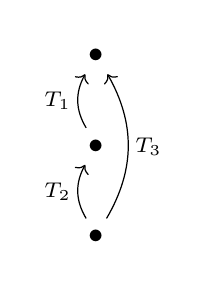
\begin{tikzpicture}

			% https://tikzcd.yichuanshen.de/#N4Igdg9gJgpgziAXAbVABwnAlgFyxMJZABgBoAmAXVJADcBDAGwFcYkQBhEAX1PU1z5CKMgEZqdJq3YBRHnxAZseAkTLEJDFm0QgA4jwkwoAc3hFQAMwBOEALZIyIHBCSiaAIxhgoSAMxOWtK6ACoA+gAs8la2Dojuzq6I5J7evogBNEE6IOF+0SA29o40LkgpIF4+SAC0mc70WIzskGBsNHAAFliWOCUgjPRejAAKAirCINZYJp19WVI5AJJhAOyG3EA
			\node[scale=1.1] (a) at (0,0){
				\begin{tikzcd}
					\bullet \\
					\bullet \arrow[u, "T_1", bend left]\\
					\bullet \arrow[u, "T_2", bend left]
					\arrow[uu, "T_3"',bend right]
				\end{tikzcd}
			};
		\end{tikzpicture}
		\label{fig:KAminor}
	\end{figure}
	The arrow between the lower and object must be the composition $T_1\circ T_2 = T_3$ because of the very definition of functor.

\end{frame}

\subsubsection{Structural constraints}
\begin{frame}
	\frametitle{Structural constraints}
	\textbf{How can we group similar musical objects together ?}
	\begin{itemize}
		\item We propose a set of candidates to be EK-nets  : $$\kappa : Hom(\Delta) \rightarrow \wp(T/I)$$
		\item The solution is the set of EK-nets $F$ such that for all arrows $a\in Hom(\Delta)$, $F(a)\in\kappa(a)$
	\end{itemize}
\end{frame}

\subsubsection{Relational Constraints}
\begin{frame}[fragile]
	\frametitle{Relational constraints}
	\textbf{How can we define relations between musical objects ?}
	\begin{itemize}
		\item We propose a set of candidates to be arrows between EK-nets $$\rho : Obj(\Delta) \rightarrow \wp(T/I)$$
		\item For two EK-net $F:\Delta\rightarrow T/I$ and $F':\Delta'\rightarrow T/I$, $F$ is in relation with $F'$ via the relational constraint $rho$ if there is an arrow $\big<N,\nu\big>$ where for all object $\delta$ of $\Delta$, $$\nu_\delta\in\rho(\Delta)$$
	\end{itemize}

	\begin{figure}
		\centering

		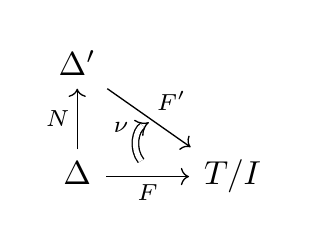
\begin{tikzpicture}

			% https://tikzcd.yichuanshen.de/#N4Igdg9gJgpgziAXAbVABwnAlgFyxMJZABgBoAmAXVJADcBDAGwFcYkQBhEAX1PU1z5CKMgEZqdJq3YBRHnxAZseAkTLEJDFm0QgA4jwkwoAc3hFQAMwBOEALZIyIHBCSiaAIxhgoSAMxOWtK6ACoA+gAs8la2Dojuzq6I5J7evogBNEE6IOF+0SA29o40LkgpIF4+SAC0mc70WIzskGBsNHAAFliWOCUgjPRejAAKAirCINZYJp19WVI5AJJhAOyG3EA
			\node[scale=1.2] (a) at (0,0){
				\begin{tikzcd}
					\Delta' \arrow[rd, "F'",""{name=Fp,right}]              &     \\
					\Delta \arrow[u, "N"] \arrow[r, "F"',""{name=F}]
					\arrow[Rightarrow , "\nu" , from=F,to=Fp, bend left=50]
					& T/I
				\end{tikzcd}
			};
		\end{tikzpicture}
		\label{fig:KAminor}
	\end{figure}

\end{frame}

\subsubsection{Pitch-classes as structural constraintsn}
\begin{frame}[fragile]
	\frametitle{Pitch-classes as structural constraints}
	\begin{columns}
		\begin{column}{0.33\textwidth}
			\begin{figure}[ht]
				\centering
				\begin{tikzpicture}[baseline= (a).base]

					\node[scale=1] (a) at (0,0){
						% https://tikzcd.yichuanshen.de/#N4Igdg9gJgpgziAXAbVABwnAlgFyxMJZABgBoA2AXVJADcBDAGwFcYkQAdDgI2ccZg4QAX1LpMufIRRkALNTpNW7Lr36CRYkBmx4CRAIyliChizaIQm8bqlEyJmmeWWRCmFADm8IqABmAE4QALZIZCA4EGE0jBAQaPakfkxwMAqM9NwwjAAKEnrSIAFYngAWQk5KFiAAKgD6wORYwtYggSFIRhFRiF2x8YYAHGTJjKnpmdl5tvqWxWUViubsAJINAEwA1i2i-kGhiOGRnTRZYFBIALQAzOHO1fWNzSAxk7n5dnMl5a3tB0c9LpnC6IW6vLLvGaFAR+Rb3VYbTaXJotGg4ehYRjsSBgNi7Nr7JDrNE9a7CSjCIA
						\begin{tikzcd}
							{}
							\bullet
							\arrow["I\_"',loop, distance=2em, in=125, out=55]  & \\
							&  \\
							\bullet
							\arrow[uu, bend right] \arrow[uu, bend left] &
						\end{tikzcd}
					};
				\end{tikzpicture}
				\caption{Structural constraint for EK relative pitch classes}
				\label{fig:constrRelPitchClass}

			\end{figure}
		\end{column}

		\begin{column}{0.34\textwidth}
			\begin{figure}[ht]
				\centering
				\begin{tikzpicture}[baseline= (a).base]

					\node[scale=1] (a) at (0,0){
						% https://tikzcd.yichuanshen.de/#N4Igdg9gJgpgziAXAbVABwnAlgFyxMJZABgBoA2AXVJADcBDAGwFcYkQAdDgI2ccZg4QAX1LpMufIRRkALNTpNW7Lr36CRYkBmx4CRAIyliChizaIQm8bqlEyJmmeWWRCmFADm8IqABmAE4QALZIZCA4EGE0jBAQaPakfkxwMAqM9NwwjAAKEnrSIAFYngAWQk5KFiAAKgD6wORYwtYggSFIRhFRiF2x8YYAHGTJjKnpmdl5tvqWxWUViubsAJINAEwA1i2i-kGhiOGRnTRZYFBIALQAzOHO1fWNzSAxk7n5dnMl5a3tB0c9LpnC6IW6vLLvGaFAR+Rb3VYbTaXJotGg4ehYRjsSBgNi7Nr7JDrNE9a7CSjCIA
						\begin{tikzcd}
							{}
							\bullet
							\arrow["I\_"',loop, distance=2em, in=125, out=55]  & \\
							&  \\
							\bullet
							\arrow[uu, bend right,"I_k"'] \arrow[uu, bend left] &
						\end{tikzcd}
					};
				\end{tikzpicture}
				\caption{Structural constraint for the $k${th} pitch classes}
				\label{fig:constrRelPitchClass}

			\end{figure}
		\end{column}
		\begin{column}{0.34\textwidth}
			\begin{figure}[ht]
				\centering
				\begin{tikzpicture}[baseline= (a).base]
					\node[scale=1.2] (a) at (0,0){
						% https://tikzcd.yichuanshen.de/#N4Igdg9gJgpgziAXAbVABwnAlgFyxMJZABgBoA2AXVJADcBDAGwFcYkQAdDgI2ccZg4QAX1LpMufIRRkALNTpNW7Lr36CRYkBmx4CRAIyliChizaIQm8bqlEyJmmeWWRCmFADm8IqABmAE4QALZIZCA4EGE0jBAQaPakfkxwMAqM9NwwjAAKEnrSIAFYngAWQk5KFiAAKgD6wORYwtYggSFIRhFRiF2x8YYAHGTJjKnpmdl5tvqWxWUViubsAJINAEwA1i2i-kGhiOGRnTRZYFBIALQAzOHO1fWNzSAxk7n5dnMl5a3tB0c9LpnC6IW6vLLvGaFAR+Rb3VYbTaXJotGg4ehYRjsSBgNi7Nr7JDrNE9a7CSjCIA
						\begin{tikzcd}
							r\arrow["I_{i+10}"',loop, distance=2em, in=125, out=55]  & &\\
							&    &  \\
							a \arrow[uu, "I_{5}"', bend right]
							\arrow[uu, "T_{i+5}", bend left] &&
						\end{tikzcd}
					};
				\end{tikzpicture}
				\caption{The 12 relative pitch classes for F}
				\label{fig:solF}
			\end{figure}
		\end{column}
	\end{columns}


\end{frame}

\subsubsection{Transpositions as relational constraints}

\begin{frame}[fragile]
	\frametitle{Transpositions as relational constraints}
	\begin{columns}
		\begin{column}{0.3\textwidth}
			\begin{figure}[ht]
				\centering
				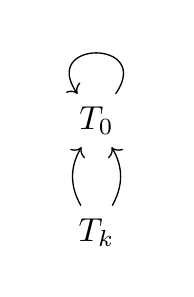
\begin{tikzpicture}[baseline= (a).base]

					\node[scale=1.2] (a) at (0,0){
						% https://tikzcd.yichuanshen.de/#N4Igdg9gJgpgziAXAbVABwnAlgFyxMJZABgBpiBdUkANwEMAbAVxiRABUB9YkAX1PSZc+QijIBGKrUYs2XANZ8pMKAHN4RUADMAThAC2ScdRwQkZEACMYYKEgDMxftr2HExkKfPVrtpAFpHZxBdA29PM0QLBggINCJxAA4yLUY4GCkGOmsGAAUhPAI2HSxVAAscJV4gA
						\begin{tikzcd}
							T_0 \arrow[loop, distance=2em, in=125, out=55] \\
							T_k \arrow[u, bend left] \arrow[u, bend right]
						\end{tikzcd}
					};
				\end{tikzpicture}
				\caption{Structural constraint for the $k^{th}$ transposition}
				\label{fig:constrRelPitchClass}

			\end{figure}
		\end{column}
		\begin{column}{0.67\textwidth}
			\begin{figure}[ht]
				\centering
				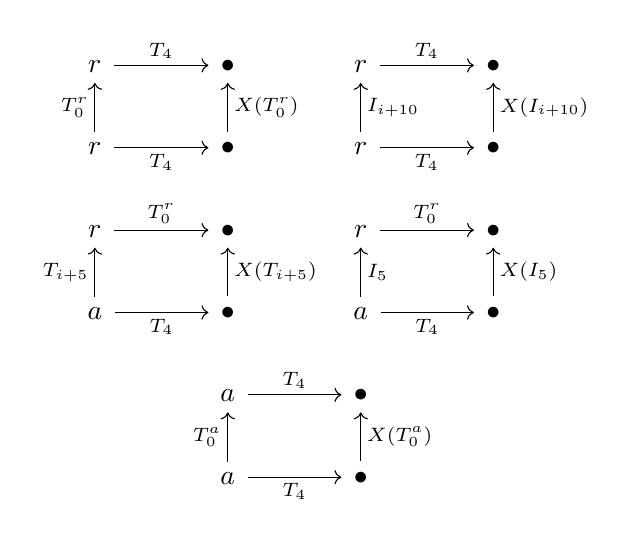
\begin{tikzpicture}[baseline= (a).base]
					\node[scale=1] (a) at (0,0){
						% https://tikzcd.yichuanshen.de/#N4Igdg9gJgpgziAXAbVABwnAlgFyxMJZARgBoAWAXVJADcBDAGwFcYkR6QBfU9TXfIRQAmCtTpNW7ADrSARs0aMYObrxAZseAkVEBWcQxZtEIWQqUq1fLYKJkDNI1NOceNgTpQAGUgGZDSRMOaw1+bSFkX2FA43YAJ1DNT0iyAKcgmXlFZVV3MNsvElIYjLjTcxyrfOSI3VJvWJcQRJrwuxFSYibg1vVajuQ-Bp6si1yk9qLh7rLmyss8-qnI4dKJcrNsxcnC1f9Riu2Jtr369ede3ZT69I3mt2WznxG5q9Obl9n796fP4u+lzGVSWHjqKDIjTewJ2XHEMCgAHN4ERQAAzeIQAC2SGGIBwECQvh+7AAKgB9bwgGiMehyGCMAAKK3YyjRoJAGOxuJoBKQohJpgp5GpIFp9KZLNMbI5XJxiGJfMQZEFIGFoTl-N5hOV0NMAA0ABQU7wASlF4oZzOeLSwiIAFrLMfLyNqkHoaXSrVKxTB2aKgULycAsABqPRcDXOpCu-E6gBserV5JFnol1s+todTu5iA9caQAHY096bfE7Y6A5kg1T8prEImC4hi6qjRSQ+GuOaS5KyxWc-KAJxuxAADiTAElg2HiN5Iz2M+Cs5W69GxyPZ0n1avc8Om8QVYHk6mxV7e5ny9mo7mDxviUejVOO7Ouxaz4uOsuB0hiPmlcRYyPKc9DfdMfUvFd1HrACNwFI8TWveViDxf84OrEBH3JPRu1PMC+yvHckL-HVkIXcD+yrTZtygtdiEbf893glNEJ-Ft-0bJjaxom82JI8dVWo9FaP4hikzbSkcMtc8lwgvJKC4IA
						\begin{tikzcd}[column sep = 1.2cm]
							r \arrow[r, "T_4"]& \bullet&
							r \arrow[r, "T_4"] & \bullet\\
							r \arrow[u, "T_0^r"] \arrow[r, "T_4"']
							& \bullet \arrow[u, "X(T_0^r)"']
							& r \arrow[u, "I_{i+10}"'] \arrow[r, "T_4"']
							& \bullet \arrow[u, "X(I_{i+10})"'] \\
							r \arrow[r, "T_0^r"]& \bullet &
							r \arrow[r, "T_0^r"]    & \bullet  \\
							a \arrow[u, "T_{i+5}"] \arrow[r, "T_4"']
							& \bullet \arrow[u, "X(T_{i+5})"']
							& a \arrow[u, "I_5"'] \arrow[r, "T_4"']
							& \bullet \arrow[u, "X(I_5)"'] \\
							& a \arrow[r, "T_4"] & \bullet&  \\
							& a \arrow[u, "T_0^a"] \arrow[r, "T_4"']
							& \bullet \arrow[u, "X(T_0^a)"'] &
						\end{tikzcd}
					};


				\end{tikzpicture}
				\label{fig:commute-sqr}
			\end{figure}
		\end{column}
	\end{columns}
\end{frame}

\begin{frame}[fragile]
	\frametitle{Transpositions as relational constraints}
	\begin{itemize}
		\item $X$ has a unique solution for $i$ fixed :
	\end{itemize}
	\begin{columns}
		\begin{column}{0.4\textwidth}
			\begin{align*}
				X(T^r_0)    & = T_0                & \\
				X(I_{i+10}) & = I_{i+10} = I_{j+6}   \\
				X(T_{i+5})  & = T_{i+1} = T_{j+9}    \\
				X(I_5)      & = I_9                  \\
				X(T^a_0)    & = T_0
			\end{align*}

		\end{column}
		\begin{column}{0.6\textwidth}
			\begin{figure}[ht]
				\centering
				\begin{tikzpicture}[baseline= (a).base]

					\node[scale=1.2] (a) at (0,0){
						\begin{tikzcd}
							r\arrow["I_{j+6}"',loop, distance=2em, in=125, out=55]  & &\\
							&    &  \\
							a \arrow[uu, "I_{9}"', bend right]
							\arrow[uu, "T_{j+9}", bend left] &&
						\end{tikzcd}
					};
				\end{tikzpicture}
				\caption{The solution $X$ which is the note A}
				\label{fig:constrRelPitchClass}

			\end{figure}
		\end{column}
	\end{columns}

\end{frame}


\section{Perspectives}
\subsubsection{Increase the EK toolbox}
\begin{frame}
	\frametitle{Increase the EK toolbox}
	Many of music theory tools can be embeded within the EK-net paradigm :
	\begin{itemize}
		\item K-nets
		\item Tonnetz
		\item Forte's interval vectors
	\end{itemize}
	\pause
	What if we change the category T/I for others category we could possibly :
	\begin{itemize}
		\item encode MIDI data
		\item encode glissandi (by using homotopy theory inside of categories)
	\end{itemize}

	All of these could be manipulated via constraints to generate something that could be surprising.
\end{frame}



\subsubsection{Compositionnal tools}
\begin{frame}
	\frametitle{Compositionnal tools}
	We showed a way to generate musical object that are in relation with another musical object.  We could :
	\begin{itemize}
		\item develop a solver of EK-constraints
		\item use Bach constraint solver
		\item create semi-generative music so that the DJ interacts more with MIDI data
	\end{itemize}
\end{frame}

\subsubsection{Develop a new constraint theory}
\begin{frame}
	\frametitle{Develop a new constraint theory}
	Following the path of Pierre Talbot thesis, we could extend his constraints formalization on lattices to categories in general.

	\begin{exampleblock}{Open question}
		Do the structural constraints form a category with relational constraints as arrows?
	\end{exampleblock}
\end{frame}


\section{Conclusion}
\listadd{\atiam}{\bf\scriptsize Gon}
\listadd{\atiam}{\bf\scriptsize Mano}
\listadd{\atiam}{\bf\scriptsize Yujia}
\listadd{\atiam}{\bf\scriptsize Alice}
\listadd{\atiam}{\bf\scriptsize Olivier}
\listadd{\atiam}{\bf\scriptsize Arthur}
\listadd{\atiam}{\bf\scriptsize Lucas}
\listadd{\atiam}{\bf\scriptsize André}
\listadd{\atiam}{\bf\scriptsize Zitian}
\listadd{\atiam}{\bf\scriptsize Hugo}
\listadd{\atiam}{\bf\scriptsize Théo}
\listadd{\atiam}{\bf\scriptsize Lydia}
\listadd{\atiam}{\bf\scriptsize Bruno}
\listadd{\atiam}{\bf\scriptsize Lenny}
\listadd{\atiam}{\bf\scriptsize Victor}
\listadd{\atiam}{\bf\scriptsize Colette}
\listadd{\atiam}{\bf\scriptsize Ninon}
\listadd{\atiam}{\bf\scriptsize Cyril}



\begin{frame}[fragile]
	\frametitle{Merci !}
	\begin{figure}
		\begin{tikzpicture}

			\newcommand{\numnodes}{18}
			\newcounter{atiamit}
			\setcounter{atiamit}{1}
			\newcommand{\atiamit}{\number\value{atiamit}}

			\renewcommand*{\do}[1]{
				\pgfmathsetmacro{\angle}{90 - (\atiamit-1)*360/\numnodes}
					\node[] (x\atiamit) at (\angle:3cm) {#1\addtocounter{atiamit}{1}};
			}

			\dolistloop{\atiam}

			\foreach \ii in {1, ..., \numnodes}{
					\pgfmathsetmacro{\prev}{int(ifthenelse(\ii==1, \numnodes, \ii-1))}
					\pgfmathsetmacro{\next}{int(ifthenelse(\ii==\numnodes, 1, \ii+1))}
					\draw (x\ii) -- (0,0) (x\prev) -- (x\ii) -- (x\next);

					\foreach \jj in {\ii, ..., \numnodes}{
							\pgfmathsetmacro{\drawoptions}{ifthenelse(
								\jj==(\ii+\numnodes/2) || \jj==\prev || \jj==\next,
								"none", "gray")}
							\path[draw=\drawoptions, thin] (x\ii) -- (x\jj);
						}
				}
		\end{tikzpicture}
		\caption{The ATIAM EK-net}
		\label{fig:constrRelPitchClass}

	\end{figure}
\end{frame}
\end{document}
